\section{Cell assembly detection method}
\label{chap:AssemblyMethod}
\begin{framed}
On the described data-set I applied a cell-assembly detection method (CAD) developed in our lab (\cite{RussoDurstewitz}) enable to detect agglomerates of neurons involved in the same encoding representation. In this section I present CAD to facilitate reading and interpretation of analysis results.\\The concept of cell-assembly was coined by Hebb (\cite{Hebb}), who described a cell-assembly as a group of neurons which, by functionally organizing into a temporally coherent set, come to represent mental or perceptual entities, thereby forming the basis of neural coding and computation. Nowadays the concept of cell-assembly is used loosely to describe a group of neurons that perform a given action or represent a given percept or concept in the brain. Thus the term cell assembly denotes in fact anything from the precise zero-phase-lag spike synchronization in a defined subset of neurons (\cite{Abeles}, \cite{Singer}, \cite{Roelfsema}, \cite{Diesmann}, \cite{Harris2003}) to temporally coherent changes in average firing rates on larger time scales (\cite{Goldman}, \cite{Durstewitz}).\\Which implies that the type of the detected assembly depends on the definition of the degree of temporal precision and coordination, varying those definition is possible to detect a plethora of spike patterns, as is shown in figure \ref{fig:CellAsseDet}.
\begin{figure}[H]
    \centering
    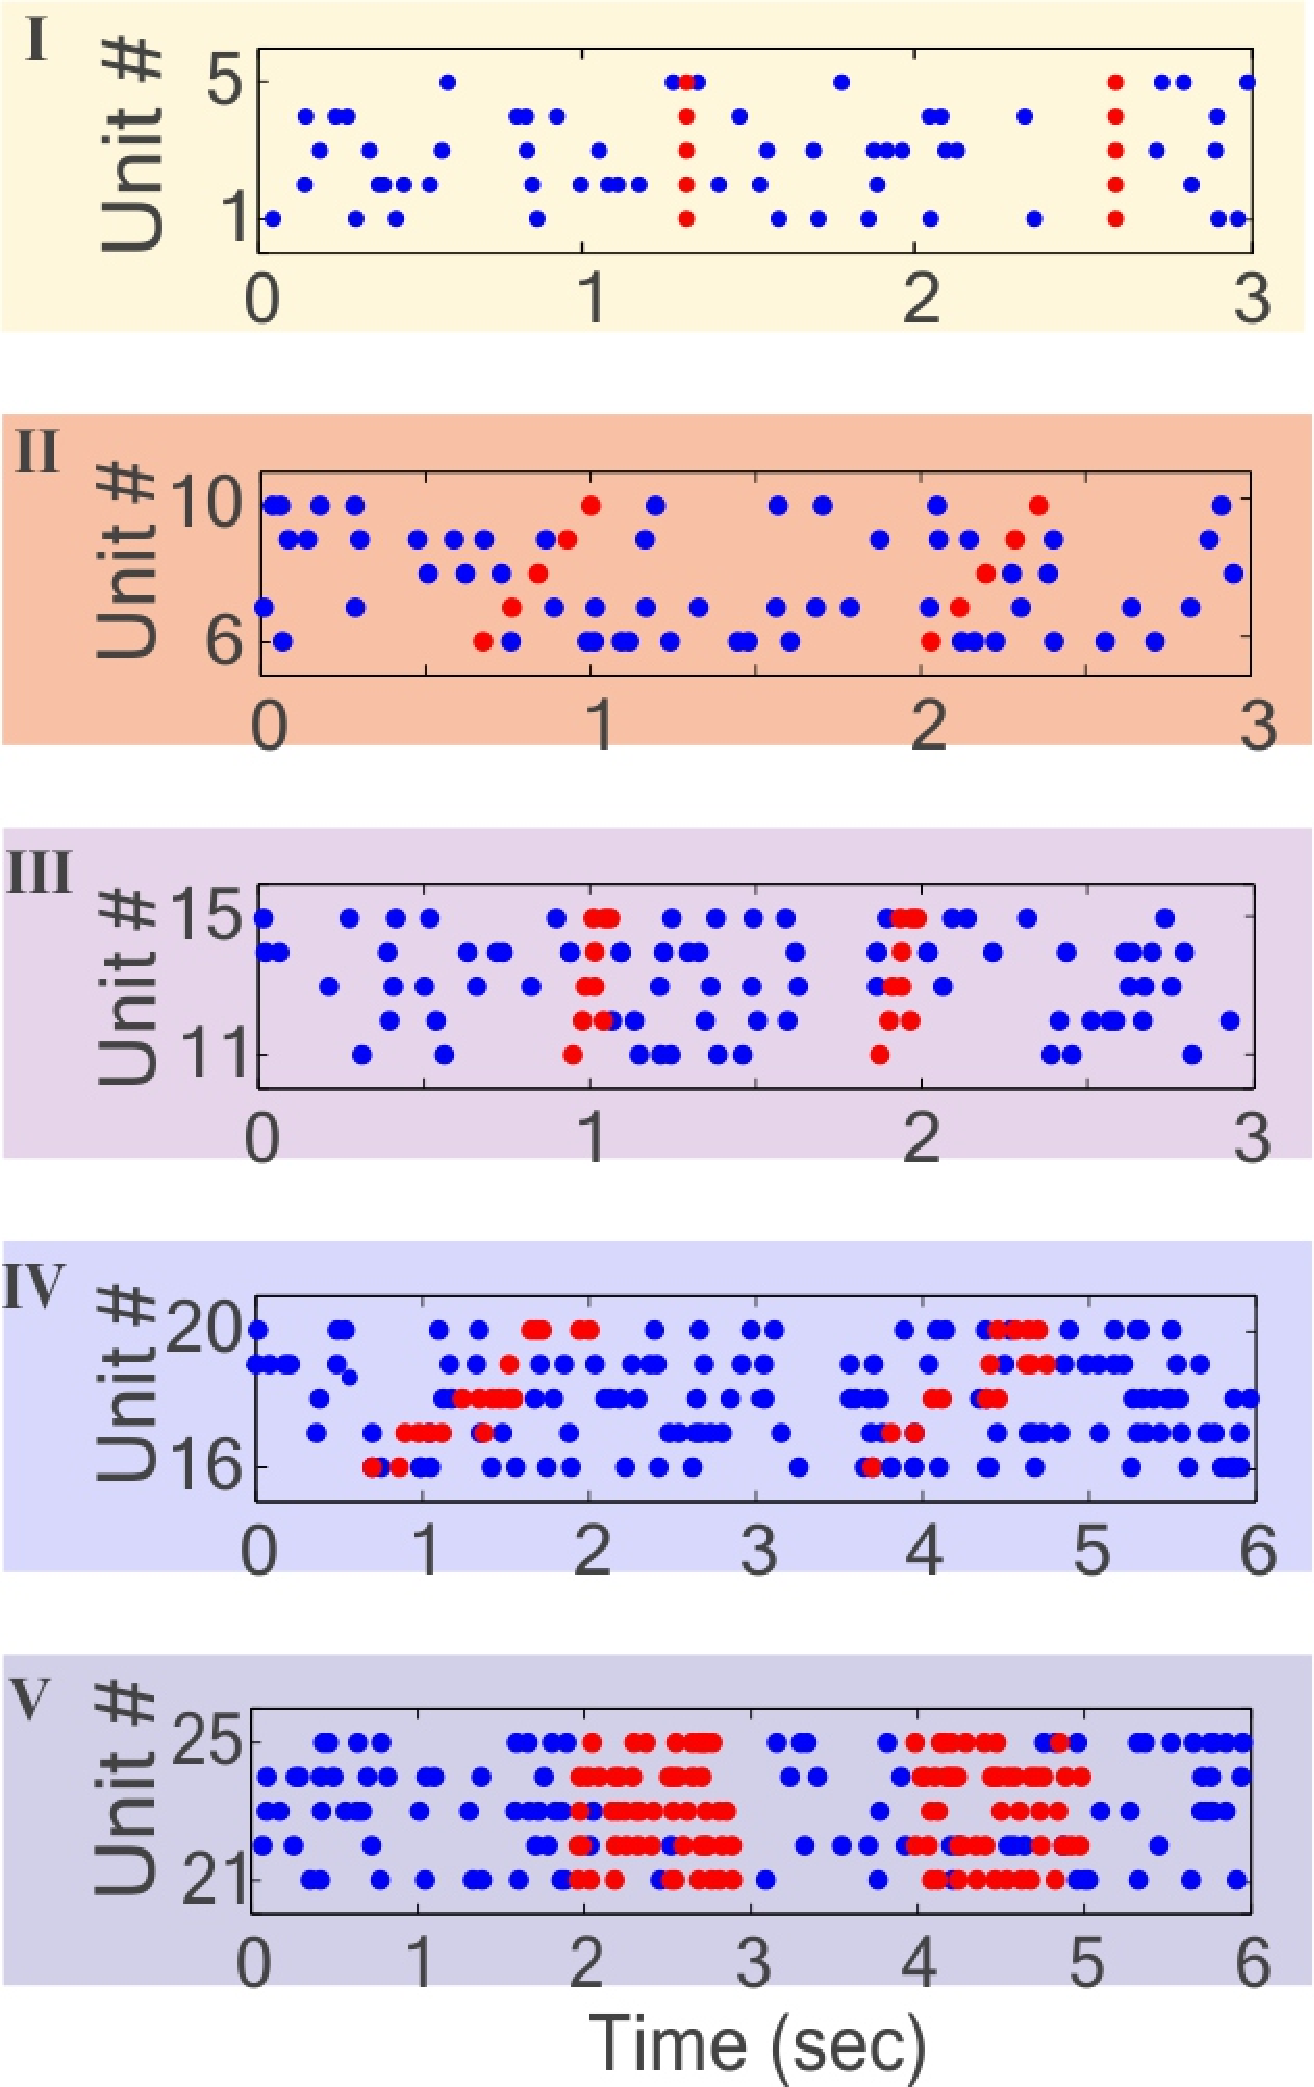
\includegraphics[scale=0.21]{figures/CellAssembliesZoom.pdf}
    \caption{Adapted from \cite{RussoDurstewitz}. Different cell assembly realizations, resulting from different definition of temporal precision and coordination.}
    \label{fig:CellAsseDet}
\end{figure}
In the recent years, neuroscientists have been invested increasing efforts to understand how cell assemblies are formed and composed, to analyse their activation and their coding (\cite{Buzsaki1}, \cite{Liu}, \cite{Cai}). This increasing interest as meant the develop of numerous mining techniques for the detection and statistical testing of cell assemblies, but most techniques limit the search for assembly patterns to one or the other specific case shown in figure \ref{fig:CellAsseDet} (\cite{Torre}, \cite{Tavoni}).\\CAD does not limit to focus on a single specific assembly concept, theoretical idea, or particular time-scale. Instead it treats the temporal scale, precision, and internal organization of coherent activity patterns as free parameters, to be determined from the data, and is thus is free to detect a large family of possible assembly definitions at any time scales and spike coordination.\\CAD is based on a statistical approach, starting from the idea that any assembly recurs as repetition of activity patterns in a set of simultaneously recorded spike trains. As shown in figure \ref{fig:CellAsseDet} a pattern of activity can be anything from synchronous and precise spike activity ($lag = 0$) to delayed spike activity ($lag\neq 0$), to broader scale of firing rate.\\Usually an arbitrary width $\Delta$ for binning the spike time series is chosen, compromising the possibility to detect any temporal scale. The idea proposed with CAD is instead to capture the multiplicity of temporal scales mentioned above introducing a set of widths $\Delta \in \{\Delta_{min},...,\Delta_{max}\}$, and retain the characteristic temporal scale of a formed assembly using a statistical test.\\CAD is conceptualized as indirect proof of not independence of the activity of units composing the assembly.\\At the first step the algorithm detects dependent pairs of units, from which high order assemblies are recursively build up using an agglomerative procedure. The mathematical formalization starts from the definition of joint probability of two independent samples.\\For two independent units with stationary spike trains, the joint distribution of spike occurrences at a specified time lag $l$ would factor into the single unit ($'$marginal$'$) distributions, $p(A,B)=p(A)p(B)$.\\ Assume each recorded spike time series has been converted into a series $\{c_t\}$ of spike counts of length T at bin width $\Delta$, with $\#_A$ and $\#_B$ denoting the total numbers of spikes emitted by units A and B, respectively. If $\Delta$ is small enough such that $c_t\in\{0,1\}$ (binary counts), then, under the null hypothesis ($H_0$) of independence, the joint spike count $\#_{AB,l}$ at time lag $l$ follows a hypergeometric distribution with mean $\mu_{AB,l}=\#_A \#_B/(T-l)$ and variance $\sigma^{2}_{AB,l}$. If the binning is such that spike counts $c_t$ larger than one occur, the hypergeometric distribution is no longer directly applicable. In this case the series are split into several (mutually dependent) binary series for which is still possible to derive a joint mean and variance (see Materials and Methods of \cite{RussoDurstewitz}).\\In principle, to proceed with the indirect proof it would be sufficient to use mean $\mu_{AB,l}$ and variance $\sigma^{2}_{AB,l}$ to check for deviation from the null hypothesis of independence $H_0$ at lag $l$, in practice such a statistic would be corrupted by non-stationarities (see Materials and Methods and Appendix of \cite{RussoDurstewitz}). Instead to use classical strategy for correcting non-stationarity such us sliding window (\cite{Gruen}) or bootstrap-based method (\cite{Fujisawa}, \cite{Pipa}, \cite{Picado}), which imply considerable computational burden, the developers of CAD alternatively suggest a new simple remedy for non-stationarity based on difference in counts $\#_{ABBA,l^-} \equiv \#_{AB,l^-} - \#_{AB,l^*}$ that subtracts from each joint spike count $\#_ {AB,l^-}$ the number $\#_{AB,l^*}$ of occurrences of the reference pattern $(A,B)_{l^*}$. Russo and Durstewitz (2017) discussed in depth the choice of the reference lag $l^*$. The statistic $Q_{AB,l}\equiv\#_{ABBA,l^2}/\hat{\sigma}_{ABBA}^2$ is approximately F-distributed and can be used for fast parametric assessment of the null hypothesis. It is important to notice that the difference statistic corrects for non-stationarity artifacts and diminish the computational load of the algorithm. This permits to test multiple bin sizes. The whole procedure is repeated for a set of user-defined bin widths $\Delta \in \{\Delta_{min},...,\Delta_{max}\}$. For each formed assembly, the width $\Delta^*$ associated with the lowest p-value is defined as its temporal precision or its typical time scale.\\CAD is particularly suited to investigate neural VS-VTA interaction involved in basal ganglia and VTA pathways in dynamic tasks such as reinforcement learning. In fact, reversal learning go/no go tasks are highly dynamic and such learning dynamic implies quick changes in network states, that can be taken in account by the cell-assembly method with the correction for non-stationarity. Moreover whilst other methods often propose to detect cell assemblies by aligning the population activity to task/behavioral events, CAD sums evidence of assembly activity throughout the task and session. This makes possible the detection of the same assembly even if its time of activation changes within the trial.
\end{framed}
